% Use wide margins, but not quite so wide as fullpage.sty
\documentclass[11pt]{article}   
\marginparwidth 0.5in 
\oddsidemargin 0.25in 
\evensidemargin 0.25in 
\marginparsep 0.25in
\topmargin 0.25in 
\textwidth 6in \textheight 8 in
% That's about enough definitions

% multirow allows you to combine rows in columns
\usepackage{multirow}
% tabularx allows manual tweaking of column width
\usepackage{tabularx}
% longtable does better format for tables that span pages
\usepackage{longtable}
\usepackage{listings}
\usepackage{graphicx}
\graphicspath{ {./images/} }

\begin{document}
% this is an alternate method of creating a title
%\hfill\vbox{\hbox{Gius, Mark}
%       \hbox{Cpe 456, Section 01}  
%       \hbox{Lab 1}    
%       \hbox{\today}}\par
%
%\bigskip
%\centerline{\Large\bf Lab 1: Security Audit}\par
%\bigskip
\author{Kinner Parikh}
\title{Lab 0: DFF and Counter}
\maketitle
\begin{center}
    CMPEN 331 - 001
\end{center}

\newpage

\section{Code}

\rmfamily
\underline{DFF Explanation:} Set output(\texttt{q}) to input(\texttt{ns}) on the positive edge of the clock and when 
the clear is on, otherwise set the output to \texttt{000}.\newline\newline
\underline{Counter Explanation:} The counter follows the diagram, in that it increments when \texttt{u} is
equal to \texttt{1} and decrements when \texttt{u} is equal to \texttt{0}. However, in the case of \texttt{u} being \texttt{1} and \texttt{ns} 
being \texttt{101}, we set \texttt{ns} to \texttt{000}, and when \texttt{u} being \texttt{0} and \texttt{ns} being \texttt{000}, we set \texttt{ns} to \texttt{101}.
And based on the current input \texttt{q}, we must change \texttt{a, b, c, d, e, f, g} to their corresponding 
defined values to represent the output on the 7-segment display.\newline\newline
\underline{Testbench Explanation:} We first define all the components of the circuit: DFF object, 
counter object, registers and wires that connect up the modules. We initially set the clear 
and clock to 0 and 1 respectively, the counter input \texttt{u} to 1, then we wait 1ms and set the
clear to 1 and 16ms later set the counter input \texttt{u} to 0. Then we have a loop where we wait 
for 1ms, then flip the clock.\newline

\ttfamily
\lstinputlisting{this.txt}

\newpage

\ttfamily
\lstinputlisting{testbench.txt}

\newpage
\rmfamily
\section{Images}

\begin{center}
    \underline{Timing Waveform}

    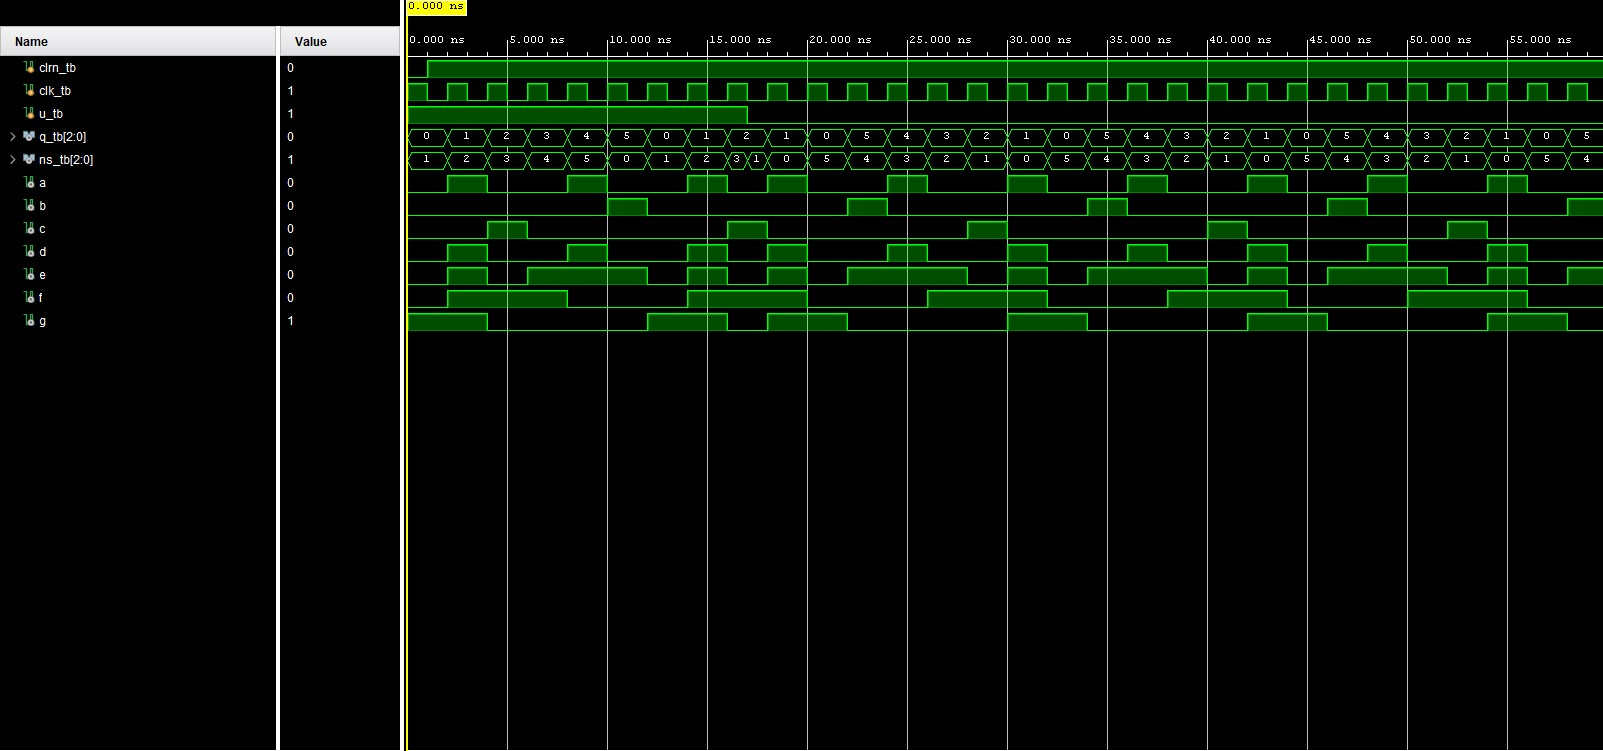
\includegraphics[width = 0.6\textwidth]{timingdiag.jpg}

    \underline{Schematic}

    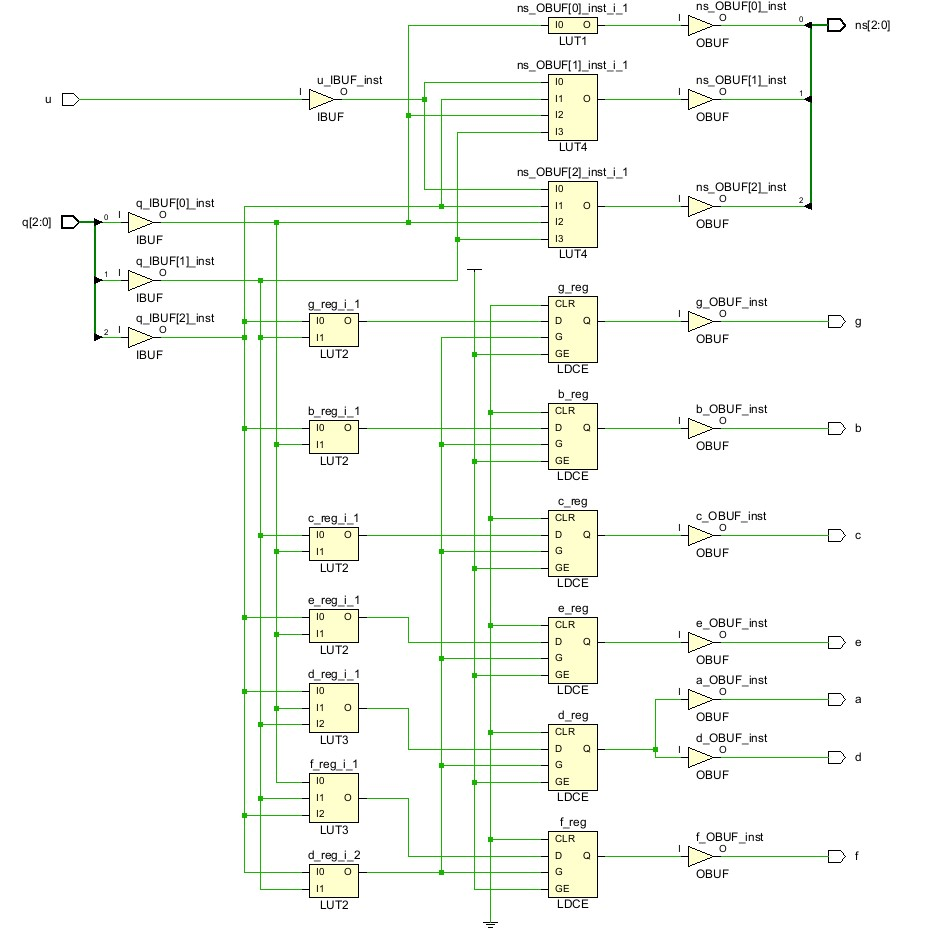
\includegraphics[width = 0.6\textwidth]{schematic.jpg}

    \newpage

    \underline{I/O Planning}

    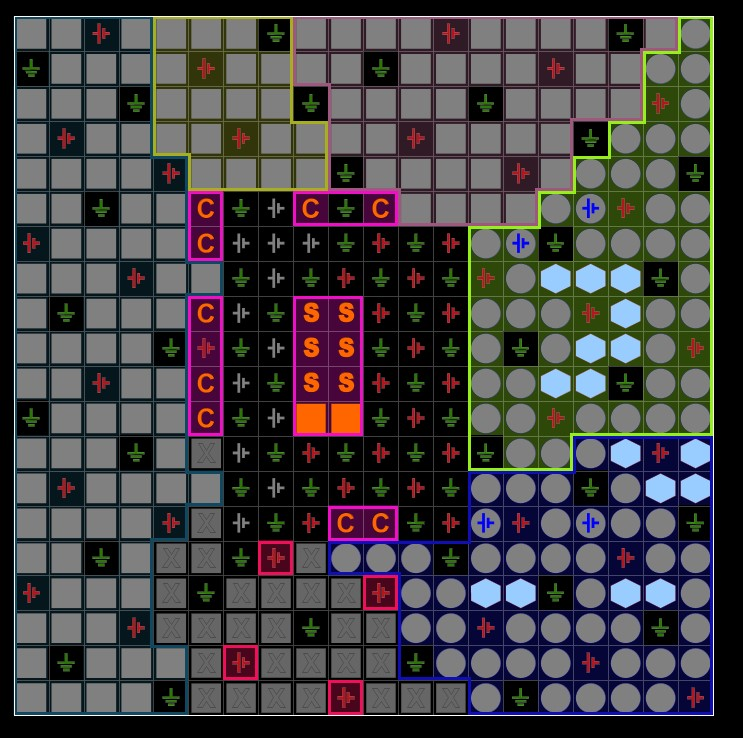
\includegraphics[width = 0.6\textwidth]{ioplanning.jpg}

    \underline{Floor Planning}

    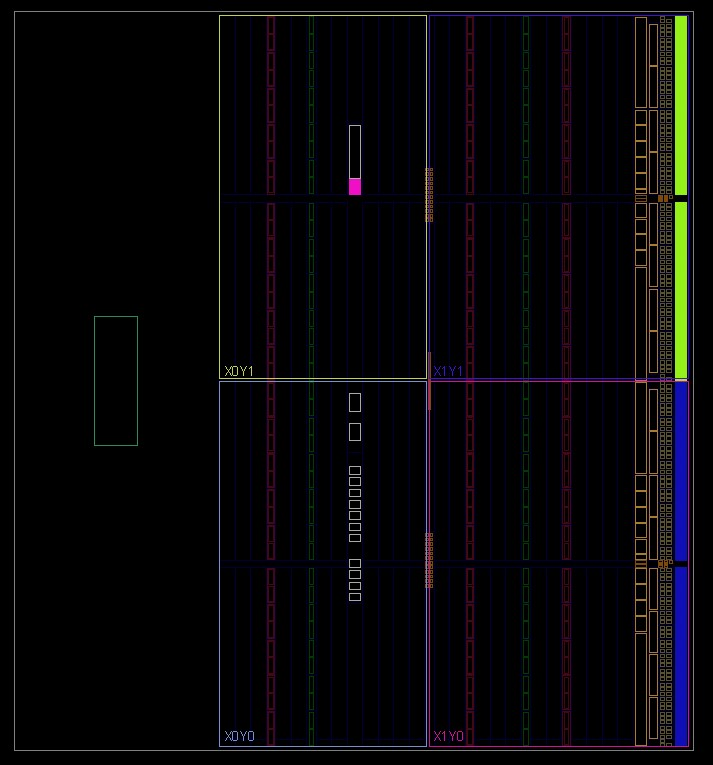
\includegraphics[width = 0.6\textwidth]{floorplanning.jpg}


\end{center}

\end{document}